%%%%%%%%%%%%%%%%%%%%%%%%%%%%%%%%%%%%%%%%
% Beamer Presentation
% LaTeX Template
% Version 1.0 (10/11/12)
%
% This template has been downloaded from:
% http://www.LaTeXTemplates.com
%
% License:
% CC BY-NC-SA 3.0 (http://creativecommons.org/licenses/by-nc-sa/3.0/)
%
%%%%%%%%%%%%%%%%%%%%%%%%%%%%%%%%%%%%%%%%%

%----------------------------------------------------------------------------------------
%	PACKAGES AND THEMES
%----------------------------------------------------------------------------------------

\documentclass[xcolor=dvipsnames, aspectratio=169]{beamer}

\mode<presentation> {

% The Beamer class comes with a number of default slide themes
% which change the colors and layouts of slides. Below this is a list
% of all the themes, uncomment each in turn to see what they look like.

\usetheme{Madrid} %Hannover
% As well as themes, the Beamer class has a number of color themes
% for any slide theme. Uncomment each of these in turn to see how it
% changes the colors of your current slide theme.
\useoutertheme{infolines} % Alternatively: miniframes, infolines, split
\useinnertheme{circles}
\definecolor{UBCblue}{rgb}{0.04706, 0.13725, 0.26667} % UBC Blue (primary)
\usecolortheme[named=UBCblue]{structure}
}

\usepackage{graphicx} % Allows including images
\usepackage{booktabs} % Allows the use of \toprule, \midrule and \bottomrule in tables
\usepackage{textpos}
\usepackage{caption}
\usepackage[utf8]{inputenc}
\usepackage[brazilian]{babel}
\usepackage{csquotes}
\usepackage{listings}
\setbeamertemplate{caption}[numbered]
\usepackage[style=abnt]{biblatex}
\addbibresource{bibliography.bib}
\PassOptionsToPackage{useregional}{datetime2}
\usepackage{xcolor}
\usepackage{amsmath}


\definecolor{codegreen}{rgb}{0,0.6,0}
\definecolor{codegray}{rgb}{0.5,0.5,0.5}
\definecolor{codepurple}{rgb}{0.58,0,0.82}
\definecolor{backcolour}{rgb}{0.95,0.95,0.92}
\definecolor{string-color}{rgb}{0.3333, 0.5254, 0.345}

\lstdefinestyle{mystyle}{
    backgroundcolor=\color{backcolour},   
    commentstyle=\color{codegreen},
    keywordstyle=\color{string-color},
    keywordstyle=[2]{\color{codepurple}},
    keywordstyle=[3]{\color{magenta}},
    numberstyle=\tiny\color{codegray},
    stringstyle=\color{codepurple},
    basicstyle=\ttfamily\footnotesize,
    breakatwhitespace=false,         
    breaklines=true,                 
    captionpos=b,                    
    keepspaces=true,                 
    numbers=left,                    
    numbersep=5pt,                  
    showspaces=false,                
    showstringspaces=false,
    showtabs=false,                  
    tabsize=2,
    otherkeywords = {tf, Sequential, SimpleRNN, Dense, GRU, LSTM},
    morekeywords = [3]{keras},
}

\lstset{style=mystyle}
\newcommand{\source}[1]{\vspace{-20pt} \caption*{ Fonte: {#1}} }
\usepackage{copyrightbox}


\makeatletter
% \beamer@nav@subsectionstyle{hide/hide/hide}
\addtobeamertemplate{sidebar left}{%
\hspace{0.5cm}
\includegraphics[width=0.9cm, keepaspectratio]{figures/_brasao_ufsm_cor.png}
% \hspace{2.3cm}
\includegraphics[width=0.8cm, keepaspectratio]{figures/brasao_ctism.png}
% \hspace{2.3cm}\includegraphics[width=1.5cm, keepaspectratio]{_logosbc.png}
% \hspace{2.3cm}\includegraphics[width=1.5cm, keepaspectratio]{_logoERRC.png}%
}{}


\setbeamertemplate{footline}
{
	\leavevmode%
	\hbox{%
	    % \hspace{0.5cm}
\includegraphics[width=0.8cm, keepaspectratio]{figures/_brasao_ufsm_cor.png}
		\begin{beamercolorbox}[wd=.333333\paperwidth,ht=2.25ex,dp=1ex,right]{date in head/foot}%
			\usebeamerfont{date in head/foot}\insertshortdate{}\hspace*{2em}
			\insertframenumber{} / \inserttotalframenumber\hspace*{2ex} 
		\end{beamercolorbox}}%
		%\vskip0pt%
	}
\makeatother

%----------------------------------------------------------------------------------------
%	TITLE PAGE
%----------------------------------------------------------------------------------------

\title[INTERNAL POSITION ERROR CORRECTION]{INTERNAL POSITION ERROR CORRECTION} % The short title appears at the bottom of every slide, the full title is only on the title page

\author[FDR]{Fábio Demo da Rosa} % Your name
%\includegraphics[]{logositeredes.png}
\institute[UFSM] % Your institution as it will appear on the bottom of every slide, may be shorthand to save space
{
Universidade Federal de Santa Maria \\ % Your institution for the title page
Pós-Graduação em Ciência da Computação \\
Disciplina de Robótica Móvel\\
\medskip
\textit{faberdemo@gmail.com} % Your email address
}
\date{\today} % Date, can be changed to a custom date
\newcounter{saveenumi}
\newcommand{\seti}{\setcounter{saveenumi}{\value{enumi}}}
\newcommand{\conti}{\setcounter{enumi}{\value{saveenumi}}}

\resetcounteronoverlays{saveenumi}


\begin{document}

\begin{frame}
\titlepage % Print the title page as the first slide
\end{frame}

\begin{frame}
\frametitle{Visão Geral} %\includegraphics[]{logositeredes.png}} % Table of contents slide, comment this block out to remove it
\tableofcontents % Throughout your presentation, if you choose to use \section{} and \subsection{} commands, these will automatically be printed on this slide as an overview of your presentation
\end{frame}

%----------------------------------------------------------------------------------------
%	PRESENTATION SLIDES
%----------------------------------------------------------------------------------------

%------------------------------------------------
\section{Introdução}
%------------------------------------------------
\begin{frame}[allowframebreaks, fragile]
  \frametitle{Introdução}
  \begin{itemize}
    \item INTERNAL POSITION ERROR CORRECTION (IPEC)
    \item Contexto de robôs móveis e desafios de dead-reckoning
      \begin{itemize}
        \item Relevância de robôs em processos de automação industrial ou tarefas repetitivas, elevando a eficiência e precisão;
        \item Dificuldades de navegação dos robôs, como deslizamento das rodas e erros acumulativos na estimativa de posição.
      \end{itemize}
    \item Objetivo do método IPEC
      \begin{itemize}
        \item Como o IPEC visa corrigir erros na estimativa da posição do robô;
        \item Aborda o aprimoramento na estimativa da direção que o robô está apontando.
      \end{itemize}
    \item Apresentação do veículo CLAPPER como caso de estudo
    \item O método IPEC realiza os seguintes cálculos uma vez durante cada intervalo de amostragem intervalo de amostragem: Primeiro, os caminhões A e B calculam sua posição e orientação momentâneas com base em
    no dead-reckoning, conforme figura abaixo:
    \newpage
    \begin{align}
      x_{A,i} &= x_{A,i-1} + U_{A,i} \cos \theta_{A,i} \\
      y_{A,i} &= y_{A,i-1} + U_{A,i} \sin \theta_{A,i} \\
      x_{B,i} &= x_{B,i-1} + U_{B,i} \cos \theta_{B,i} \\
      y_{B,i} &= y_{B,i-1} + U_{B,i} \sin \theta_{B,i}
    \end{align}
      
    \item \textbf{Onde:}
      
    \begin{itemize}
      \item \(x_{A,i}, y_{A,i}\) - Posição do ponto central do caminhão A no instante \(i\).
      \item \(x_{B,i}, y_{B,i}\) - Posição do ponto central do caminhão B no instante \(i\).
      \item \(U_{A,i}, U_{B,i}\) - Deslocamentos incrementais dos pontos centrais dos caminhões A e B durante o último intervalo de amostragem.
      \item \(\theta_{A,i}, \theta_{B,i}\) - Orientações dos caminhões A e B, respectivamente, calculadas a partir do dead-reckoning.
    \end{itemize}      
    \newpage
    \begin{figure}
      \centering
      \copyrightbox[b]{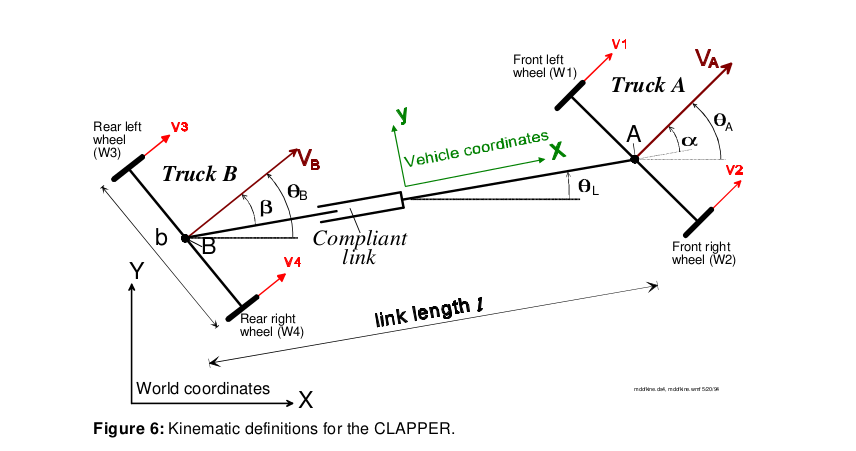
\includegraphics[scale=0.32]{figures/1_Kinematic_definitions_for_the_CLAPPER.png}}%
      {Fonte: \cite{borenstein1995intemal}}
      \caption{Definições cinemáticas para o CLAPPER.}
      \label{fig:1_Kinematic_definitions_for_the_CLAPPER}
    \end{figure} 
  \end{itemize}
\end{frame}

%------------------------------------------------
\section{Correção de Erros Translacionais}
%------------------------------------------------
\begin{frame}[allowframebreaks, fragile]
  \frametitle{Correção de Erros Translacionais}
  \begin{itemize}
    \item O método IPEC pode detectar apenas erros rotacionais e não erros translacionais. 
    \begin{itemize}
      \item Erros rotacionais são mais graves do que erros translacionais;
      \item Erros de orientação causam crescimento ilimitado de erros de posição lateral.
    \end{itemize}
        
    \item Existem dois tipos de erros translacionais: 
    \begin{itemize}
      \item Erros puros ocorrem quando ambas as rodas passam por obstáculos de altura similar, e são raros. 
      \item Erros compostos acontecem quando apenas uma roda passa por um obstáculo, causando um erro translacional e um rotacional.
    \end{itemize}
        
    \item O erro de orientação em dead-reckoning normalmente é causado por um encoder reportando uma distância horizontal maior do que a distância real percorrida pela roda,
    \begin{itemize}
      \item permitindo assim a correção através da rotação corretiva em torno do ponto de contato da roda esquerda.
    \end{itemize} 
    \newpage
    \begin{figure}
      \centering
      \copyrightbox[b]{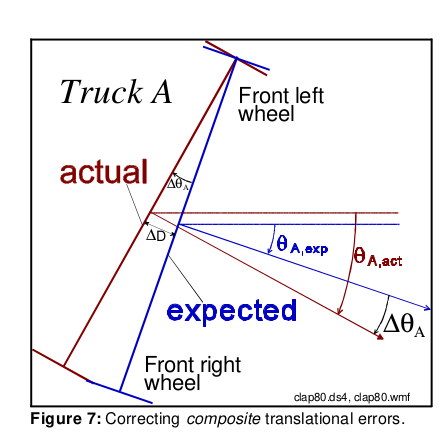
\includegraphics[scale=0.32]{figures/2_correcting_composite_translational_errors.png}}%
      {Fonte: \cite{borenstein1995intemal}}
      \caption{Correção de erros translacionais compostos.}
      \label{fig:2_correcting_composite_translational_errors}
    \end{figure} 
    \item A posição acumulada do caminhão B é sempre calculada em relação a A, usando os três codificadores internos. A única desvantagem é a necessidade de medir com precisão a distância entre os caminhões para evitar erros sistemáticos durante as curvas.
  \end{itemize}
  
\end{frame}

%------------------------------------------------
\section{Experimentos}
%------------------------------------------------
\begin{frame}{O Experimento da Linha Reta}
  \begin{columns}
    % Coluna para a figura
    \begin{column}{0.5\textwidth}
      \begin{figure}
        \centering
        \copyrightbox[b]{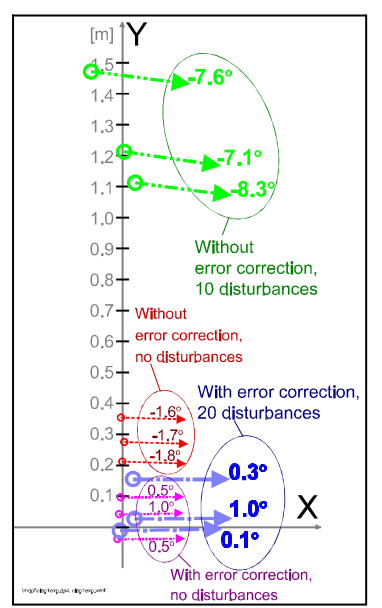
\includegraphics[scale=0.26]{figures/3_Return_position_errors_after_completing_the_Straight_Path_Experiment.png}}%
        {Fonte: \cite{borenstein1995intemal}}
        \caption{Pontos de retorno finais do experimento.}
        \label{fig:3_Return_position_errors_after_completing_the_Straight_Path_Experiment}
      \end{figure}  
    \end{column}

    % Coluna para o texto
    \begin{column}{0.5\textwidth}
      \begin{itemize}
        \item O CLAPPER percorreu 18m para a frente e voltou 18m para trás.
        \item "sem obstáculos", o piso do laboratório é liso para evitar perturbações.
        \item "com obstáculos", apenas as rodas do lado direito encontraram os obstáculos.
        \item \textbf{Com} correção de erro (IPEC), foram usados 20 obstáculos espaçados uniformemente pelo caminho de retorno.
        \item \textbf{Sem} correção de erro, foram usados apenas 10 obstáculos devido ao espaço limitado do laboratório.
      \end{itemize}      
    \end{column}
  \end{columns}
\end{frame}

\begin{frame}{O Experimento do Caminho Retangular}
    \begin{columns}
      % Coluna para a figura
      \begin{column}{0.5\textwidth}
        \begin{figure}
          \centering
          \copyrightbox[b]{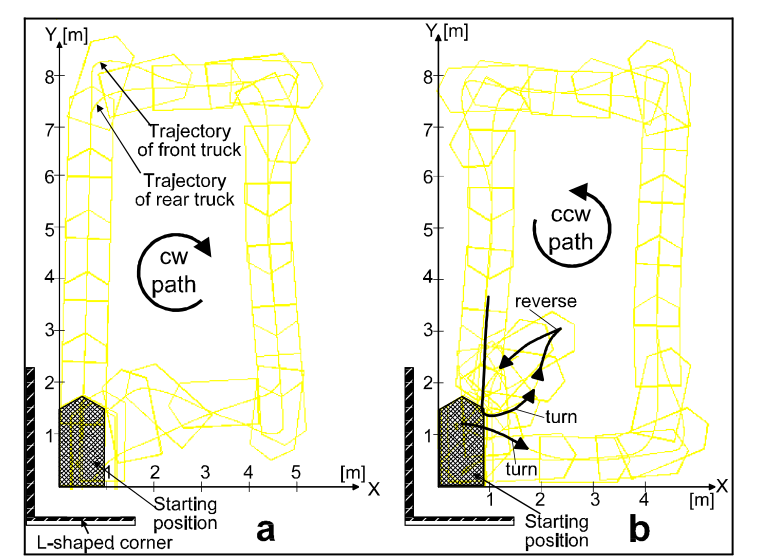
\includegraphics[scale=0.28]{figures/4_The_Rectangular_Path_Experiment.png}}%
          {Fonte: \cite{borenstein1995intemal}}
          \caption{Rectangular Path Experiment.}
          \label{fig:4_The_Rectangular_Path_Experiment}
        \end{figure}  
      \end{column}
  
      % Coluna para o texto
      \begin{column}{0.5\textwidth}
        \begin{itemize}
          \item O CLAPPER seguiu um caminho retangular de 7x4 m com curvas suaves de 90 graus, sem parar nos cantos.
          \item Testes foram feitos em ambas as direções (cw e ccw) para evitar compensação mútua de erros sistemáticos.
          \item 10 corridas em cada direção, com e sem obstáculos, produziram erros de posição não superiores a 5 cm.
          \item O método IPEC resultou em uma redução de mais de 20 vezes nos erros de orientação.
        \end{itemize}      
      \end{column}
    \end{columns}
  \end{frame}

%------------------------------------------------
\section{Conclusões}
%------------------------------------------------
\begin{frame}{Conclusões}
  \begin{itemize}
    \item Resumo das contribuições do método IPEC.
      \begin{itemize}
        \item Eficácia na correção de erros sistemáticos e não-sistemáticos em tempo real;
        \item Versatilidade de aplicação em veículos com diferentes graus de liberdade.
      \end{itemize}
    \item Importância da correção imediata dos erros.
      \begin{itemize}
        \item Redução significativa do retrabalho;
        \item Melhoria considerável na confiabilidade do sistema de navegação.
      \end{itemize}
    \item Validade do método em diferentes cenários.
      \begin{itemize}
        \item Aplicação em ambientes industriais;
        \item Utilidade em ambientes com irregularidades no solo, como na construção e na agricultura.
      \end{itemize}
    \item Aplicabilidade Futura do Método IPEC.
      \begin{itemize}
        \item Extensão para outros tipos de configurações de veículos, como a adição de um reboque codificador não motorizado;
        \item Possibilidade de uso em robôs móveis colaborativos mas fisicamente desconectados, equipados com sensores de posição precisos.
      \end{itemize}
  \end{itemize}
\end{frame}



%------------------------------------------------
%\section*{Referências}
%------------------------------------------------
\begin{frame}
    % \nocite{*}
    \printbibliography
\end{frame}


\begin{frame}
\titlepage % Print the title page as the first slide
\end{frame}

\end{document}